
\documentclass[journal]{IEEEtran}

\usepackage{graphicx}
\usepackage[utf8]{inputenc}
\usepackage{algorithm}
\usepackage{algorithmic}
\usepackage{amsmath}
\usepackage{amssymb}
\usepackage{caption}
\usepackage{xcolor}

\captionsetup[figure]{font=small,labelfont=small}

\begin{document}
 
\title{\textbf{counteracting learnability imbalance in multiclass-classification}}

\author{Theodor Peifer
        \linebreak
        email: thp7219@thi.de
        \linebreak
        Technische Hochschule Ingolstadt
}

\maketitle

\begin{abstract}
Neural Networks have proven themselves to be powerful classification
models by solving problems in a range of domains with high accuracy.
Yet this accuracy is never evenly distributed across all classes, which means that the true-positive rates of each class separately are different.
%This can happen even in balanced datasets since some classes are more difficult to learn by the model than others (this phenomenon is further referred to as \emph{learnability-imbalance}).
%This research will investigate if and how the moethods to counteract class imbalance can be adapted to the more general problem of learnability imbalance.
%A more severe version of this problem appears when working with class imbalance, for which are already methods existing.
Although this problem is most common and severe when working with class imbalanced datasets, it can also occur with balanced datasets.
This is because there are always classes which are more difficult for the model to learn than others (this phenomenon is further referred to as \emph{learnability-imbalance}).
This research will examine whether and how the methods to counteract class imbalance can be adapted to the more general problem of learnability imbalance.
% Since those methods use the different class proportions as a measure for how much they should affect each class, they are not directly appliable when working with balanced datasets. %they can not be applied to datasets with classes that have the same amount of samples.
% Therefore, this research will propose an approach in which a model gets pre-trained normally and then the true positive scores of this model are used to train the model independently again but usng the class imbalance methods based based on the evaluation scores, instead of the class sizes.
Since those methods use the different class proportions as a measure of how much they should affect each class, this research will propose approaches, which are also applicable on balanced datasets.
%The main approach is to use the true-positive scores of a previously normally trained model as a measure, rather than the class sizes.
%In that approach the methods on class imbalance are used but by using the true positive rates of a pre-trained model instead of the different class sizes.
% (i.e. the categories the model has to classify between)
%Since those methods rely on knowing the different class proportions, we propose a way to calculate how much a methods should affect each class by using the true positive score
%This research will address the determination of such weights to counteract the learnability-imbalance in balanced datasets using previously calculated evaluation scores.
%Therefore the goal is to find methods to lower the variance of the true positive rates of each class.
\end{abstract}


\section{Introduction}
A frequent problem in classification appears when working with datasets that have an unequal amount of samples per class and are therefore called a \emph{class imbalanced} datasets. %, where \emph{classes} describe the categories which the model has to classify.
Since there will be some classes, that have less elements for the model to learn from, their features will be harder to extract what finally will result in a lower true positive rate, i.e. a per-class accuracy.
Thus, the consequence of having different class sizes can be described as having a \emph{learnability imbalance} in the dataset, since some classes are more difficult to learn that others.

But such learnability differences can appear also in balanced datasets for a variety of reasons, e.g. when the quality of the data of a class is lower than the rest of the data. % or when the classes come not from the distributions. 
A second reason, that this research will be focusing on, is that when some classes are similiar,
the model can confuse their samples with each other more easily which will often result in a lower accuracy of those classes.

Even though this issue is an inevitable product of every normal classification, in most cases the learnability difference of the classes is either low or not from great interest.
But there can be more extreme cases in which a model needs to produce fair and unbiased results using a dataset that has an obvious learnability imbalance. 
An example for that is \emph{name-ethnicity classification}, where a model predicts the ethnicity of a name only by its letters [5]. 
Nationalities that use the same language and therefore have similiar names (e.g. \emph{british} and \emph{american}) result in a lower accuracy (see figure 1).
Thus, when a model that is trained on such a dataset is used, e.g. for social science experiments, it can lead to unfair results and wrong interpretations. 

\begin{figure}[h!]
        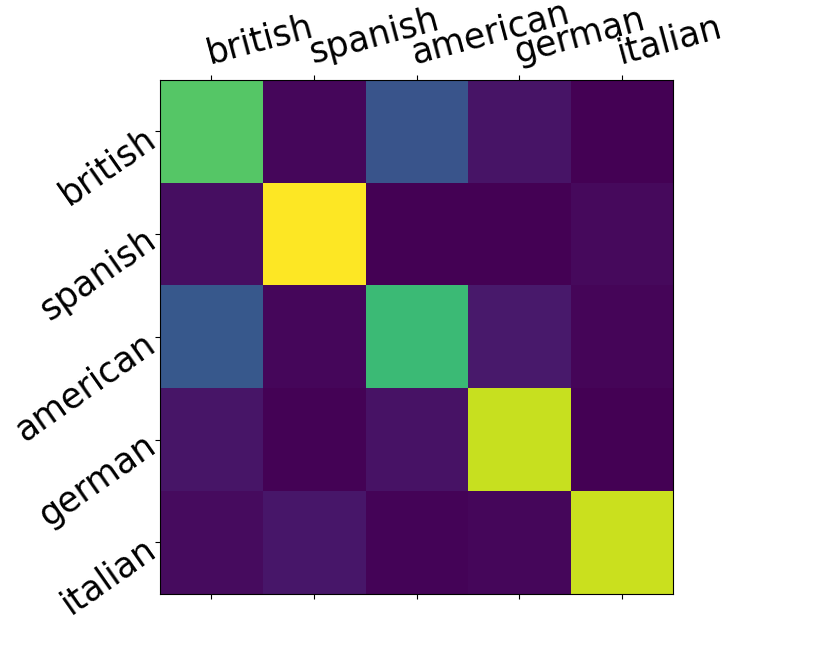
\includegraphics[width=\linewidth]{images/Figure_1.png}
        \caption{A confusion matrix representing the true positive distribution of the name-nationality dataset produced by a recurrent neural network and the confusion of british and american names}
        \label{fig:tp_scores}
\end{figure}

Another dataset that is a good showcase for the learnability imbalance is the CIFAR-10 [2] dataset (32$\times$32 RGB images of ten different classes) because it also contains similiar classes such as \emph{dog} and \emph{cat}.
The CIFAR-10, a name-nationality and a further tabular dataset will be used for experiments in order to find methods for minimizing the variance in the evaluation scores.

To find out such methods, one should first resort to the solutions of the class imbalance problem.
One of them is the weighting of the error function [1] according to the size of each class, i.e. the number of samples it contains.
Therefore, there is a weight assigned to every class, which is greater the fewer elements it contains and that gets multiplied with the loss produced by its samples. % "Therefore" wrong
That will cause, that samples from a smaller class will produce a higher error and, since the aim of a neural network is to minimize the error [4], will receive a higher focues in the learning process.
Other methods will be discussed in the literature review.

But almost all of the approaches to counteract class imbalance rely on the different proportions of the classes in the dataset. 
This raises the question if and how they are applicable on datasets that, even though they don't suffer from class imbalance, still show a big learnability imbalance.
When working with such datasets the learnability differences of the individual classes are mostly only identifiable after the model has been trained normally und unweighted. % and without any regard for the potential imbalance of the dataset. 
The calculation of the true positive rates and a visualization (e.g. confusion matrix) can then reveal what classes were learned the best and which should have received a higher weight.
These evaluation scores can then be used, for example to determine which loss weights should be used for each class (an example is shown in \emph{algorithm 1}).

\begin{algorithm}[H]
        \caption{creating loss weights for a balanced dataset}

        \textit{\textbf{C} $\hat{=}$ amount of classes}
        \\ \textit{\textbf{train(weights)} describes the initialization and training process of a classification model in which $weights_i$ will be multiplied to every loss generated by a sample of class $i$.}
        \\ \textit{\textbf{evaluate()} creates the set $s$ with $\left|s\right|$ = $C$ and $s_i \in [0;1]$ which contains the true positive scores of all classes of the test dataset.}
        \\ \textit{\textbf{W(s)} is a function that creates a set of loss-weights $w$ with $\left|w\right|$ = $C$ and $w_i \in \mathbb{R}^{+}$ using a set of true positive scores $s$: $W: [0;1] \rightarrow \mathbb{R}^{+}$ ; $\{s_i,...,s_C\} \rightarrow \{w_i,...,w_C\}$ }
        \\ \textit{\textbf{process:}}
        \begin{algorithmic}[1]
         \STATE $train(weights\texttt{=}\{w_1\texttt{=}1, w_2\texttt{=}1, ..., w_C\texttt{=}1\}$)
         \STATE $s = evaluate()$
         \STATE $w = W(s)$
         \STATE $train(weights\texttt{=}w)$
         \STATE $s' = evaluate()$
         \STATE $compare(s, s')$

        \end{algorithmic}
\end{algorithm}

In summary, this research will focus on adapting the methods, that are used to counteract class imbalance, to the learnability imbalance problem of balanced datasets.
This will be done by using the true positive rates produced by the evaluation of an independently pre-trained model.
Instead of class sizes, these rates will be used as a measure for how much a method should affect each class.

\begin{figure}[h!]
        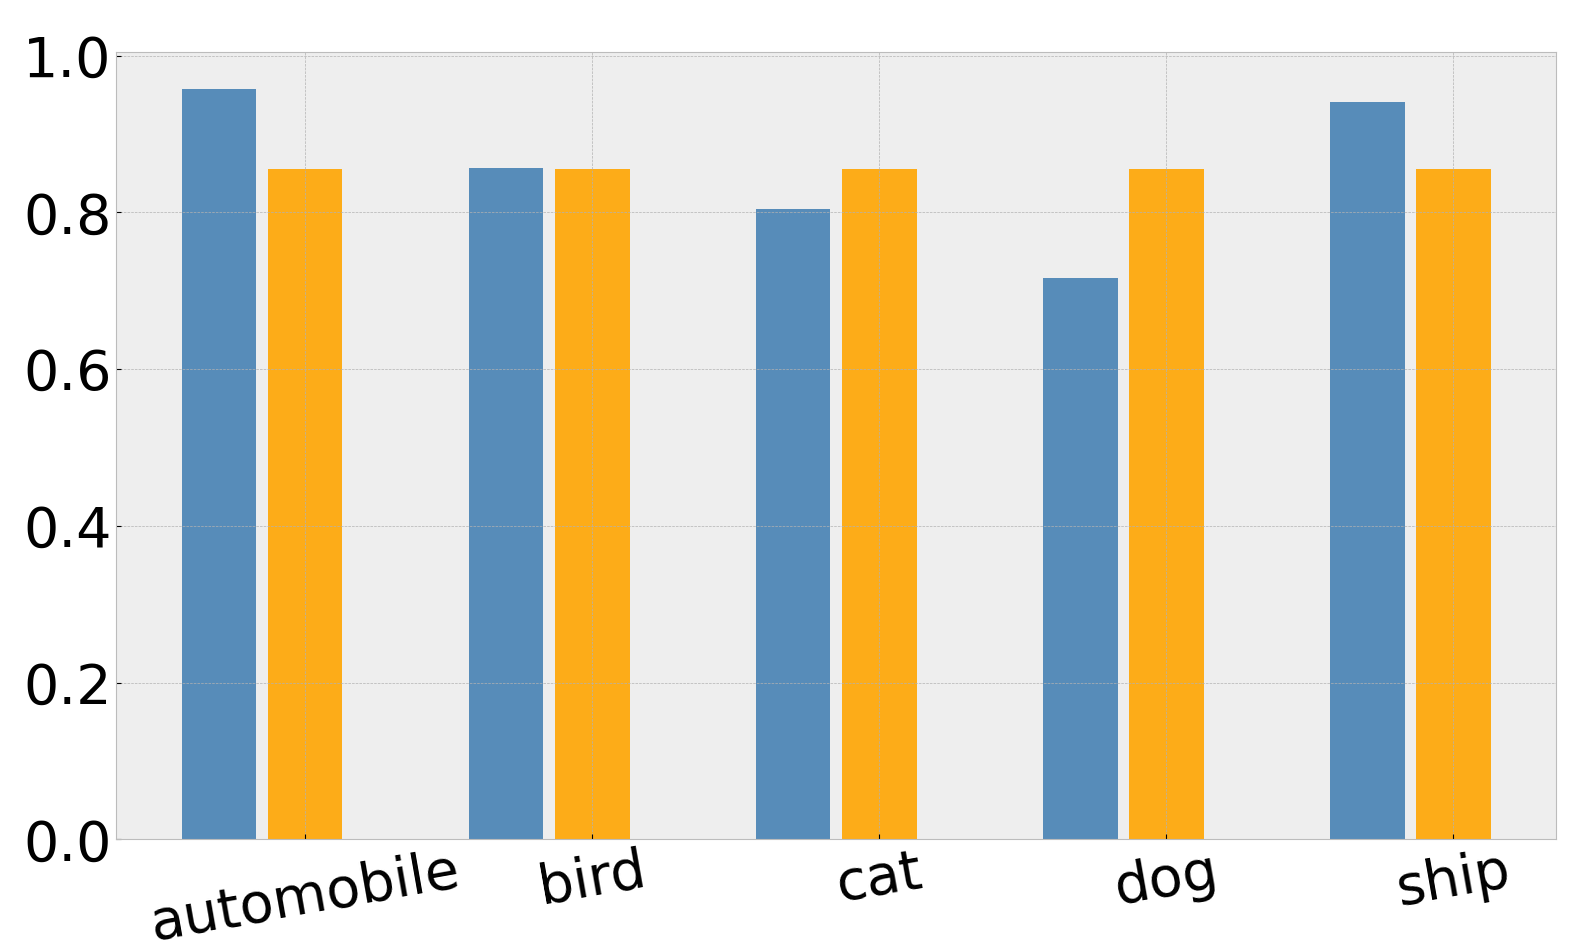
\includegraphics[width=\linewidth]{images/tp_comparison.png}
        \caption{true positive rates produced by a model that was trained normally (\textcolor{blue}{blue}) on five CIFAR-10 classes compared to the desired true positive rates (\textcolor{orange}{orange})}
        \label{fig:tp_comparsion}
\end{figure}

The aim of the research is to find approaches that bring all per-class accuracies to nearly the same value by increasing those of classes that are harder to learn 
and decrease them of classes that are more easily to learn without the reduction of the overall accuracy (see figure 2).
Further, it will address potential limitations and risks that could potentially happen from this process.

\section{literature review}
As mentioned before, the learnability imbalance has to be handled the same way as the class imbalanced dataset problem, but by using the true positive rates instead of the class proportions of the dataset.
Therefore, the proposed solutions to class imbalance are fundamental to this research and will be reviewed in the following (the methods in summary: loss weighting, augmentation and over-/ undersampling).

Since it was used as a main example in the introduction, the first method to examine is loss weighting. 
This approach has proven itself to be a good way for archieving a lower variance in the per-class accuracies of unbalanced datasets and will be adapted to this research. 
In general, the weights are chosen to be inversely proportional to the amount of samples in the classes [Na], in order to weight smaller classes more than bigger ones. 
An example for a weight calculation function, proposed by Yin Cui et al. (2019) [N], is shown in forumla 1:

\[ w_c = \frac{1-\beta^{N_c}}{1-\beta} \]

\emph{further normalization:}

\[ w_c = \frac{C * w_c}{\sum_{i=1}^{C}w_i} \]

This method gets described as the \emph{effective number of samples} weighting, where $N_c$ is the amount of samples of class $c$ and $\beta$ is a tuneable hyper-parameter with $\beta \in [0;1[$ .

Formula 2 shows how to use such weights along with the cross entropy loss function [N] for one sample:

\[ \text{CE}(x, c) = w_{c} \cdot \left(-\log\left(\hat{y}_c)\right) \right) \]

$\hat{y}$ is the output of a model $\text{F}(x, \theta)$ with input sample $x$ and learnable parameter $\theta$. 
It be described as a probability distribution for which $\hat{y_i}$ is the confidence of the model, that the input $x$ corresponds to the $i$-th class.
Therefore $\hat{y_c}$ represents the probability that the model correctly classified $x$ as the wanted class $c$. 
As shown, the weight $w_c$ that corresponds to the correct class gets multiplied with the normal error value (in the case of cross entropy: the negative $\log$ of the probablity).

Another loss weighting method is the so called \emph{focal loss} and was introduced by Tsung-Yi Lin et al. (2018) [N] in order to handle class imbalance in object detection.
This approach is especially interesting for this research because it uses the true positive rates instead of the sizes of the classes to generate the weights and can therefore be applied unchanged to the learnability imbalance problem.
But since it is also mainly tested and practiced with class imbalanced datasets, this research will investigate its effectiveness on class balanced datasets that have high learnability variances.
The weight for the focal loss is defined as the following ($\gamma$ is a positive hyperparameter for scaling):
\[ w_c = (1 - \hat{y}_c)^\gamma \]

When multiplying this weight with the loss, it will be bigger, the smaller the confidence of the correct class was. 
The adavantage of the focal loss over the proposed weight generation of this research is that it does not require a pre-training in order to figure out which classes a harder to learn, since it does this during the training process.
But it can be hypothized that this weighting could have less impact on learnability imbalanced datasets because it figures out the imbalance while training.
In contrast to this, when training unweighted first, calculating the weights afterwards and then train again with those weights, the loss function can start penalizing the classes differently right from the beginning.

Another method is \emph{augmentation} [N], in which the input samples get randomly modified in order to synthetically generate more training samples and therefore help the model to generalize better. 
For example, in image classification it is common to flip, crop or to add white noise to the images. 
The idea, originally proposed as \emph{SMOTE} (Synthetic Minority Over-sampling Technique) by Nitesh V. Chawla et al. (2002) [N], is that such transformations can be used on smaller classes to provide the model with more of their samples.
The same technique can be used on learnability imbalanced datasets but by applying it on classes with a lower per-class accuracy.

% \begin{figure}[h!]
%         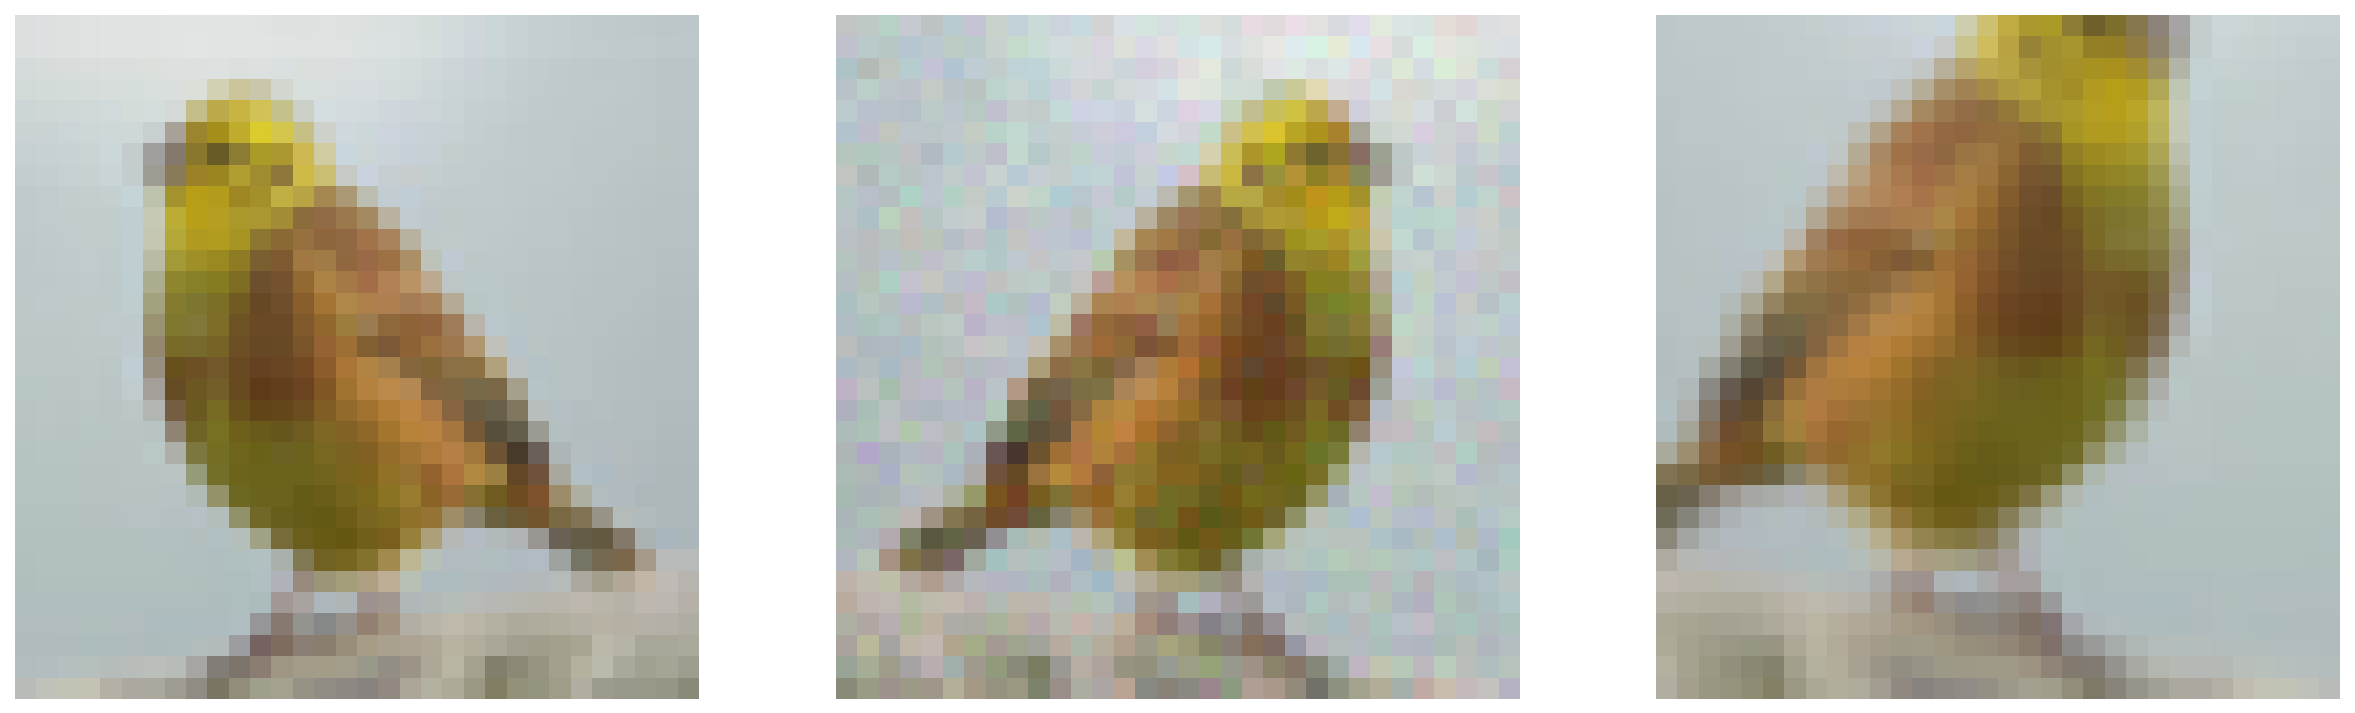
\includegraphics[width=\linewidth]{images/augmentation3.png}
%         \caption{An example of augmentation applied on a CIFAR-10 32$\times$32 image using the "imgaug" Python libary [N] (ltr: flip, gaussian noise, crop)}
%         \label{fig:augmentation}
% \end{figure}

Another way to try to compensate for class imbalance is by doing \emph{oversampling} [N] where the model gets fed samples of the minority classes more often.

Even though \emph{undersampling} (the ignoring of samples of big classes) is also an option in extreme cases, it is more likely to have an negative impact on the learnability imbalance.
That's because, when reducing the size of easier to learn classes, it will probably result in the decrease of their accuracy without an increase of the accuracy of the other classes.
This hypothesis will also be checked in this research.

From the approaches mentioned above, the focal loss is the only one that can be tested on balanced datasets as it is. 
The others require a pre-training in order to determine the learnability differences and therefore the true positive rates, which then can be used to estimate or calculate how much these methods should affect each class.

\section{methodology}
In order to produce appropriate results, the proposed approach has to be applied on different models with different tasks. 
There are three main diciplines: image, sequential data and tabular data classification. 
When testing the approach on each task, the results can be interpreted more generalized. 
But it can also reveal if any methods works better for one specific dicipline than for others. 
If there is such a suspicion, the methods will be tested on more datasets.

As already mentioned in the introduction, to test the approaches on image classification the CIFAR-10 dataset will be used.
It contains 60.000 32$\times$32 pixel RGB (i.e. channels for red, green and blue color) images, that are equally distributed among ten classes.
This dataset is freely available and commonly used in computer vision research.
The architecture of the model that will be trained on this dataset will be a convolutional neural network with residual connections [N].
For testing the approach on sequential data, a private name-ethnicity dataset will be used.
This dataset was gathered by the government of United Kindom Of Great Britain and provided to the author for a prior collaboration project based on name-ethnicity-classification.
Within this project, the maximum accuracy for this classification problem was reached by using a \emph{ConvLSTM} architecture [N], i.e. the combination of a convolutional neural network and a LSTM (long-short term memory) [N], which will also be used in this research. 
Finally, the tabular dataset that will be used is the ------ dataset which contains of --------------- with --- classes.

The metric used for measuring how much a potential learnability imbalance impacted the model is the variance of the per-class accuracies.
Therefore, the effectiveness of the proposed approaches can be determined by the difference between the variances generated with and without the approaches.

\[ Var(s) = \frac{1}{C} \sum_{i=1}^{C} (s_i - \bar{s})^2 \]
\[ D = Var(s) - Var(s') \]

$s'$ are the true positive scores produced by a model using one of the proposed methods and $s$ of a model that was trained normally. 
If $Var(s')$ is smaller that $Var(s)$, a approach showed a potential effectiveness.
But if the difference is not significant, a statistical test must be performed in order to investigate if the reason for this difference was indeed the used method.

The experiments will be implemented in the \emph{Python} programming language and the models will be built and trained using the \emph{Pytorch} deep learning framework [N].
In addition, an experiment manager, such as \emph{Weights\&Baises} [N], will keep the results in an orderly and accessible manner.

\section{research plan}
This research is expected to be completed in a little over a year and will not consume many ressources.
The reason for that is that the capacities (i.e. number of parameters) of the models used for the experiments are not high, since they don't need to reach state-of-the-art results.
Additionally, the datasets (which are already provided) are not particularly high dimensional and consist of a manageable amount of samples.
Therefore the experiments do not require high-end hardware and can be run in a short amount of time.

The esitmated duration of this research is 14 months and will be performed in four stages, as shown in the table below.

\begin{center}
        \captionof{table}{schedule of research} 

        \begin{tabular}{ |c|c|c|c| } 
                \hline
                stage & description & duration \\
                \hline
                %\multirow{3}{4em}{Multiple row} & cell2 & cell3 \\ 
                1 & investigation & 4 months \\ 
                2 & execution & 5 months \\ 
                3 & revision & 2 months \\ 
                4 & writing & 3 months \\
                \hline

        \end{tabular}
\end{center}
        
In the first stage, the investigation, theoretical approaches are conceptualized by doing a more indepth literature review and adapting the proposed approaches to the learnablity imbalance problem. 
The aim is to find several candidates for functions that produce loss weights, augmentation chances and oversampling amounts based on the true positive scores.
This investigation gives also the opportunity to encounter previously unconsidered methods with which the research can be extended.

The execution stage will begin by setting up the project code repository (link [N]). 
It will contain the model architectures, train scripts and implementations of the conceived methods.
Then the experiments will be run, the results collected and finally analyzed. 

In the next stage, the revision, the used approaches and the results will be reviewed and compared. 
After this process is finished, the last stage, the writing of the research paper can begin. 
Presumably after three months, the paper can be submitted and is ready for reviewing.  


\begin{thebibliography}{1}

\bibitem{}
Name Name, Name Name, Name Name (2006). Title, 24(1), 29-33.

\end{thebibliography}

\end{document}

% biased class distribution: https://link.springer.com/chapter/10.1007/3-540-44795-4_45#:~:text=Labeled%20data%20for%20classification%20could,optimal%20classification%20on%20new%20data.
% class imbalance over sampling: https://machinelearningmastery.com/random-oversampling-and-undersampling-for-imbalanced-classification/
% CEL: https://arxiv.org/ftp/arxiv/papers/2001/2001.00570.pdf
% a: https://arxiv.org/pdf/1901.05555.pdf (p 4)
% focal loss: https://arxiv.org/pdf/1708.02002.pdf
% smote: https://arxiv.org/pdf/1106.1813.pdf